%%%%%%%%%%%%%%%%%%%%%%%%%%%%%%%%%%%%%%%%%%%%%%%%%%%%%%%%%%%%%%%%%%%%%%%%%%%%%
\chapter{Infos About \LaTeX{} / Your Thesis}\label{chap:info_REMOVE_ME}
%%%%%%%%%%%%%%%%%%%%%%%%%%%%%%%%%%%%%%%%%%%%%%%%%%%%%%%%%%%%%%%%%%%%%%%%%%%%%
\chapterstart

\chapquote{Research is formalised curiosity. It is poking and prying with a purpose.}
          {Zora Neale Hurston}
          
Each chapter should start with a short explanation what is inside the upcoming chapter and why it has been included (at this position) in your work: This template shall provide some considerations\footnote{
In addition to the references at the end of this chapter, consider recommended ways of writing learnt in the lecture \emph{Scientific Writing}. Find the official requirement-documents as well as supporting material at the E-Learning platform.
} 
and text examples for your Bachelor's or Master's thesis.


\section{About this chapter}
Selected \LaTeX{} examples.

\subsection{Examples for named paragraphs}

% example for a named paragraph
\paragraph{Background.}
Describe the background, the prerequisites for your work \ldots

\paragraph{Objective.}
The aim of this master's thesis is \ldots

\paragraph{Terms and definitions.}
Technical terms \ldots\ abbreviations are summarised at the end (in Chapter~\ref{chap:acronyms} ``\nameref{chap:acronyms}''), e.g.\ \ac{ABI} or \ac{MITM}. If \ac{ABI} is referenced again, only the acronym is printed (as hyperlink though).

\subsection{About Research Resources}
For literature research\footnote{You might start your search at URL \url{http://dl.acm.org/} or \url{http://ieeexplore.ieee.org/}.} use e.g. \citetitle{acm:diglibrary} \parencite{acm:diglibrary} or \citetitle{ieee:xplore} \parencite{ieee:xplore} as available from the FH JOANNEUM Libary web page.

\subsection{About Citation Styles}
Harvard citation style is implemented in this template. For information about a topic like RFID paraphrased in your own words~\citep[cf.][pg 317]{Batina:2011} do not forget to use \emph{cf.} and -- if available the relevant page numbers -- along with \emph{citep}. Direct quotations would not need the \emph{cf.}. If you need to use the title of a reference, for example the RFID Authentication Protocol by \citet{Fernandez-Mir:2011} you might use \emph{citet}. For references without parentheses (find more in \cite{Li:2008}) just use \emph{cite}.

Note the use of \emph{ibid} (in German \emph{ebd} or \emph{ebenda}) for referencing (several pages of) the same resource subsequently. For example, see \citep[cf.][pg 317]{Batina:2011} and \citep[cf.][pg 321]{Batina:2011} \citep[cf.][pg 399]{Batina:2011}.

You might cite URLs, e.g. about (tools for checking) Accessibility~\citep[cf.][]{Google:2017a,Google:2016a}, as online resources with a date of your last visit.


\section{Some more \LaTeX}
%----------------------------------------------------------------------------
This section is a \textit{really very short} summary of \LaTeX\ features. Do not forget to remove it after finishing your thesis.

Here you have an included graphic (Figure~\ref{fig:engine}). Note the short title used for the list of figures.

\begin{figure}[h]
  \centering
  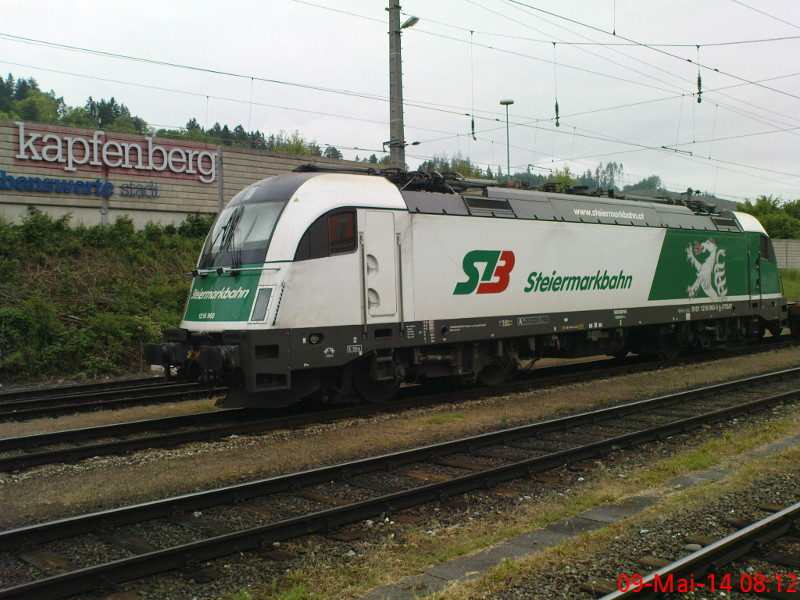
\includegraphics[keepaspectratio,width=0.95\textwidth]{images/engine}
  \caption[Logo at the train engine.]{Note the logo attached to the train engine spotted in Kapfenberg main station.}
  \label{fig:engine}
\end{figure}

Code listings require the \textit{listings} package which, in turn, requires some settings\footnote{\ldots because the defaults do not fit all purposes}; see command \verb+\lstset{}+ in preamble of this template. Additionally the package \textit{courier} should be used because the defaults do not provide for proper syntax highlighting.

\lstset{
caption={Listing subtitles could and should contain whole sentences describing the important aspect of the listing.}, 
basicstyle=\small\ttfamily, label=lst:main, language=C,frame=single}
%	basewidth={0.55em}, fontadjust}	% adjust these for more appealing appearance
\begin{lstlisting}
void main(int argc, char *argv[])
{
  printf("Hello world!");
}
\end{lstlisting}

In order to see what's possible -- here are two fancy tables, see Table~\ref{tab:olive} and Table~\ref{tab:grey} which show \ldots.

\begin{center}
  \begin{table}[tbp]
    \begin{tabular}{|l|l|l|l|}\hline
      \rowcolor{olivegreen30}
      \textcolor{white}{\textbf{Version}}
      	 &\textcolor{white}{\textbf{Description}}	
      	   &	\textcolor{white}{\textbf{Author(s)}}	
      	     &\textcolor{white}{\textbf{Date}}\\
      \hline
      1.0	
        & Initial				
          & Ohrt					
            & July 15, 2014\\
      \hline
      1.1	
        & Filled section ``Open Issues''	
          & Ohrt					
            & July 16, 2014\\
      \hline
      1.2	
        & Added section ``Restrictions''	
          & Ohrt					
            & September 15, 2014\\
      \hline
    \end{tabular}
    \caption{Olive green heading used for this fancy table.}
    \label{tab:olive}
  \end{table}
\end{center} 
  
View also the preamble of this file for explanations.
  
\begin{center} 
  \begin{table}[tbp]
    \begin{tabular}{ l | l }
      \rowcolor{gray20}\textbf{Error}	
        & \textbf{Solution} \\
      \rowcolor{gray5}Java.lang.OutOfMemoryError: PermGen space
        & -XX:MaxPermSize=1024M \\
      \rowcolor{gray5}\textit{(32-/64-bit issue)}
      	& \\
      \rowcolor{gray20}Error occurred during initialization of VM \textit{or}
      	& increase or remove -Xms value \\
      \rowcolor{gray20}Could not reserve enough space for object heap
      	& e.g.\ -Xms128m -Xmx512m \\
      \rowcolor{gray20}					
        & \small{(Eclipse default:}\\
      \rowcolor{gray20}					
        & \small{-Xms40m -Xmx512m)} \\
    \end{tabular}
    \caption{A more or less simple grey table. Better try to put tables and figures at \textit{top}[t] or \textit{bottom}[b] (optional use whole \textit{page}[p]) of a page. Avoid location specifier \textit{here}[h].}
    \label{tab:grey}
  \end{table}
\end{center}



Here is a reference to Listing~\ref{lst:main}. Note the line numbers. Referenced listings, tables and figures are written in uppercase first letter: \emph{L}isting X,  \emph{T}able Y and  \emph{F}igure Z.



\subsection{Prototype}

Find in Listing~\ref{lst:democlosure} an example of the JavaScript closure. Only parts of the original source code have been included. That allows to extract and display parts of working code!

\lstinputlisting[language=JavaScript,
 float=tbp,
 label=lst:democlosure, 
 firstline=10, 
 lastline=88, 
 caption={Demo implementation of a JavaScript \emph{Closure}.}
]{src/closure.js}

Mathematical expressions are rendered beautifully by \LaTeX. Now enjoy the first Maxwell equation 
\begin{math} 
  \text{rot} \vec{H} = \vec{J} + \frac{\partial \vec{D}}{\partial t} 
\end{math}.

Selected resources about scientific working: 

\begin{itemize}
  \item \emph{\citetitle{Zobel:2004}}: \ldots elements of good writing - clarity, simplicity, accuracy, and organization \ldots by \cite{Zobel:2004}.
  
  \item \emph{\citetitle{Yin:2013}}: \ldots offers comprehensive coverage of the design and use of the case study method as a valid research tool \ldots by \cite{Yin:2013}.

  \item \emph{\citetitle{Strunk:2000}}: \ldots first edition about 1935; includes a list of valuable recommendations: be clear, do not overwrite \ldots by \cite{Strunk:2000}.

  \item \emph{\citetitle{Field:2003}}: \ldots Planning an Experiment,	
Experimental Designs, Descriptive Statistics, Inferential Statistics \ldots Answering the Question 'So What?' \ldots by \cite{Field:2003}.

  \item \emph{\citetitle{Booth:2008}}: \ldots What Is Research? Creating a Relationship with Your Reader: Your Role, Finding a Good Research Problem \ldots by \cite{Booth:2008}.

  \item \emph{\citetitle{Alley:1998}}: 
  \ldots 
  your writing is the principle way in which people learn about your work.
  When you communicate well, you receive credit for your 
  \ldots 
  by \cite{Alley:1998}.

  \item \emph{\citetitle{Eco:2010}}: \ldots Warum muss man eine wissenschaftliche Abschlussarbeit schreiben und was ist sie? \ldots by \cite{Eco:2010}.

  \item \emph{\citetitle{Wisconsin:2004}}: \ldots you will find many instructional materials we've developed for our Writing Center teaching: Planning and Writing Research Papers, Creating an Argument,  \ldots by \cite{Wisconsin:2004}.


\end{itemize}

Finally, before starting to write you might take a look at some of these references.

\vfill

Final note: at the end of each chapter you might sum up the contents of the chapter in a sentence or two. Then you might tell the reader what will be presented in the upcoming section (to make her/him curious).


% next chapter: start at right side, if two-sided; else just flush page
\chapterend
